\chapter{Desenvolvimento}
\label{chapter:desenvolvimento}

Este capítulo aborda os seguintes tópicos:
\begin{itemize}
\item Na Seção 3.1, descrevemos a metodologia utilizada.
\item Na Seção 3.2, os resultados são mostrados e discutidos.
\end{itemize}

\section{Métodos}

%Foi planejado e realizado um estudo que visa avaliar estado manutenibilidade
%do Linux Kernel, utilizando o sofware SonarQube para a medição. Os
%requerimentos necessários pelo método SQALE foram as fornecidas pelo
%plugin \textbf{sonar-cxx\cite{Sonarcxx2016}}. O software realiza
%uma leitura completa do código fonte da aplicação a ser analisada,
%identificando os trechos não adequados de acordo com os requerimentos
%definidos. Para cada não conformidade encontrada, há uma função de
%remediação definida com o tempo estimado de remediação cada ocorrência
%encontrada. Foram consideradas 6 versões de lançamento estáveis foram
%analisadas dentro das versões mais recentes, procurando avaliar o
%estado atual da manutenibilidade do software. 
Para cada aplicação, o mesmo procedimento foi realizado. Utilizando os repositórios do sistema de controle de versão \textit{Git}[INSERIR NOTA DE RODAPE] de cada projeto, foram analisadas todas as versões marcadas como lançamentos (utilizando o sistema de marcações do sistema de versão - \textit{tags}) em que o número da versão não fosse inferior ao atual, evitando assim que o analises fossem realizadas em versões de manutenção, que possuem evolução paralela.
Como teste preliminar, usaremos o Hadoop, desenvolvido pela Apache Foundation e largamente utilizado. Foram analisadas as versões de lançamento sequências do software. As métricas mostradas são presentadas como uma função do tempo, assim como adotado em \cite{israeli2010linux}, devido a grande variância de lançamento de versões menores. Por exemplo, uma versão nomeada "2.1.1" pode ser lançada após o lançamento de uma versão "3.0.0". Portanto, utilizar as métricas como funções de números de verões pode levar a resultados enganosos.


\section{Resultados e Discussão}

Nesta seção analisamos as Leis de Evolução de Software de Lehman usando como base dados obtidos do Apache Hadoop, assim como em estudos anteriores\cite{israeli2010linux,lehman1996laws,lehman1980programs}. Assim como utilizado em \cite{israeli2010linux}, a ordem de apresentação das leis inicia com aquelas mais diretamente relacionadas ao código, assim como o agrupamento de leis que estão relacionadas.

\subsection{Lei 1: Mudança Contínua}

\begin{hypothesis}
	O número de mudanças cumulativas em cada release é diferente de zero.
\end{hypothesis}
\subsection{Lei 2: Complexidade Crescente}

\begin{hypothesis}
	A complexidade ciclomática total aumenta com o tempo.
\end{hypothesis}
\begin{hypothesis}
	A complexidade ciclomática relativa aumenta com o tempo.
\end{hypothesis}
\subsection{Lei 3: Auto-Regulação}

\begin{hypothesis}
	O número de releases com ajustes negativos ao número de funções é diferente de zero.
\end{hypothesis}
\begin{hypothesis}
		O número de releases com ajustes positovos ao número de funções é diferente de zero.
\end{hypothesis}

\subsection{Lei 4: Conservação da estabilidade Organizacional}
\begin{hypothesis}
	O número de médio de mudanças por dia é invariante.
\end{hypothesis}
\begin{hypothesis}
	A taxa de mudança ao longo do tempo decresce.
\end{hypothesis}
\begin{hypothesis}
	A taxa de crescimento ao longo do tempo decresce.
\end{hypothesis}
\subsection{Lei 5: Conservação da Familiaridade}

\begin{hypothesis}
	O crescimento dos módulos é invariante.
\end{hypothesis}
\begin{hypothesis}
	A taxa de mudança de funções decresce com o tempo.
\end{hypothesis}
\begin{hypothesis}
	O taxa de mudanças decresce com o tempo.
\end{hypothesis}

\subsection{Lei 6: Crescimento Contínuo}
De acordo com esta lei, um programa deve ser constantemente incrementado ao longo do tempo para satisfazer usuários. Aqui, "crescimento" é interpretado como o tamanho do software. O tamanho pode também ser utilizado ou indicador de funcionalidade, assumindo-se que código adicional é escrito para a criação novas funcionalidades.
\begin{hypothesis}
	O número de linhas de código cresce com o tempo.
\end{hypothesis}
\begin{hypothesis}
	O número de módulos cresce com o tempo.
\end{hypothesis}
\begin{hypothesis}
	O número de funções cresce com o tempo.
\end{hypothesis}
Tal lei pode ser validada calculando métricas de tamanho (como número de módulos) e observando sua evolução com o tempo, assim como usado por Lehman e outros estudos. Várias métricas pode ser utilizadas para descrever o tamanho de um software. Para o objeto de nossa análise utilizamos linhas de código não em branco e não comentadas, número de funções e classes para descrever o crescimento do projeto.

Ambos levam a resultados similares
\begin{figure}
	\centering
	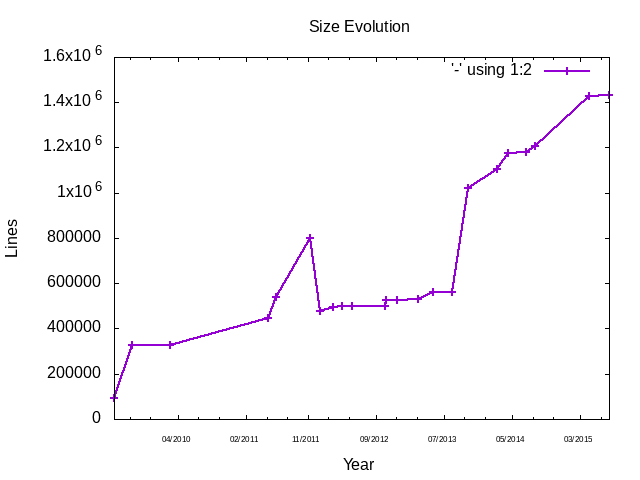
\includegraphics[width=0.7\linewidth]{figure/Lines}
	\caption{Crescimento em Linhas}
	\label{fig:lines}
\end{figure}


\begin{figure}
	\centering
	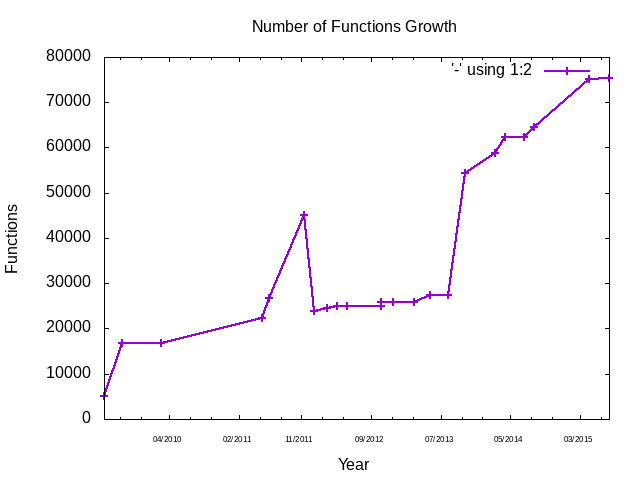
\includegraphics[width=0.7\linewidth]{figure/Functions}
	\caption{Crescimento em número de funções}
	\label{fig:function_growth}
\end{figure}



\begin{figure}
	\centering
	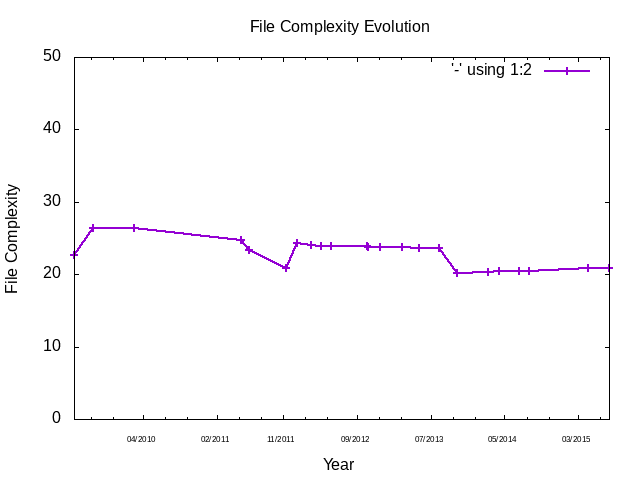
\includegraphics[width=0.7\linewidth]{figure/file_complexity}
	\caption{Evolução da complexidade/Arquivo}
	\label{fig:file_complexity}
\end{figure}

\subsection{Lei 7: Qualidade Decrescente}

\begin{hypothesis}
	A qualidade interna decresce com o tempo.
\end{hypothesis}


\begin{figure}
	\centering
	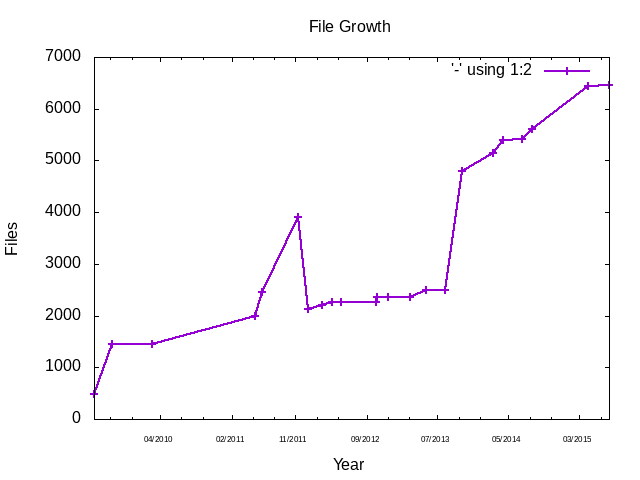
\includegraphics[width=0.7\linewidth]{figure/Files}
	\caption{Crescimento em número de arquivos}
	\label{fig:files}
\end{figure}


\subsection{Lei 8: Sistema de Realimentação}

\begin{hypothesis}
	O número de módulos: $\alpha\sqrt[3]{RSN} $
\end{hypothesis}
\begin{hypothesis}
	O número de módulos cresce com o tempo.
\end{hypothesis}
\begin{hypothesis}
	O número de funções cresce com o tempo.
\end{hypothesis}

